\documentclass[10pt]{beamer}

\usetheme[progressbar=frametitle]{metropolis}
\usepackage{appendixnumberbeamer}
\usepackage{multicol}
\usepackage{booktabs}
\usepackage[scale=2]{ccicons}
\usepackage[style=authoryear]{biblatex}
\bibliography{demo.bib}
\usepackage{pgfplots}


\usepgfplotslibrary{dateplot}


\usepackage{xspace}
\newcommand{\themename}{\textbf{\textsc{metropolis}}\xspace}

\title{Hospital Information Technology and Physician Response}

\subtitle{Hanna Glenn}
 \date{\today}
% \date{}
%\author{Presented by: Hanna Glenn}
% \institute{Center for modern beamer themes}
% \titlegraphic{\hfill\includegraphics[height=1.5cm]{logo.pdf}}

\begin{document}

\maketitle

\setbeamercolor{background canvas}{bg=white}

\begin{frame}{Table of contents}
  \setbeamertemplate{section in toc}[sections numbered]
  \tableofcontents%[hideallsubsections]
\end{frame}

\section[Motivation]{Motivation}

\begin{frame}{The Beginning of HIT}
\centering
    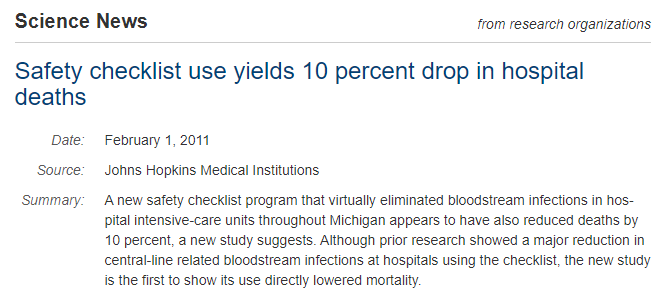
\includegraphics[scale=.6]{graphics/News Clip4.PNG}
\end{frame}

\begin{frame}[fragile]{HIT has had Great (Expected) Potential in Healthcare}
\begin{alertblock}{Cost Saving}
\begin{itemize}
    \item A 2005 estimate finds possible cost reduction of hundreds of billions of dollars (\cite{hillestad2005})
\end{itemize}
\end{alertblock}

\begin{alertblock}{Quality Improvement}
\begin{itemize}
    \item Patient safety improvements, physicians have decision support that could prevent unnecessary complications, etc.
    \item Significant policy push for EHR implementation with this goal in mind: HITECH Act, 2008 provided financial incentive for hospitals to implement EHRs \nocite{hitech}
\end{itemize}
\end{alertblock}

\textcolor{blue}{The percentage of hospitals with basic EHR capability rose from 9$\%$ in 2008 to 84$\%$ in 2015.} (\cite{stats})

\end{frame}

\begin{frame}[fragile]{What does this mean for physicians?}
\begin{itemize}
    \item Day-to-day, this means physicians spend more time entering information into a computer
    \item Loss of autonomy as EHRs have progressed
    \item Physicians have experienced significant burn-out from EHRs
\end{itemize}

\end{frame}

\begin{frame}{Physician Burnout}
\begin{center}
    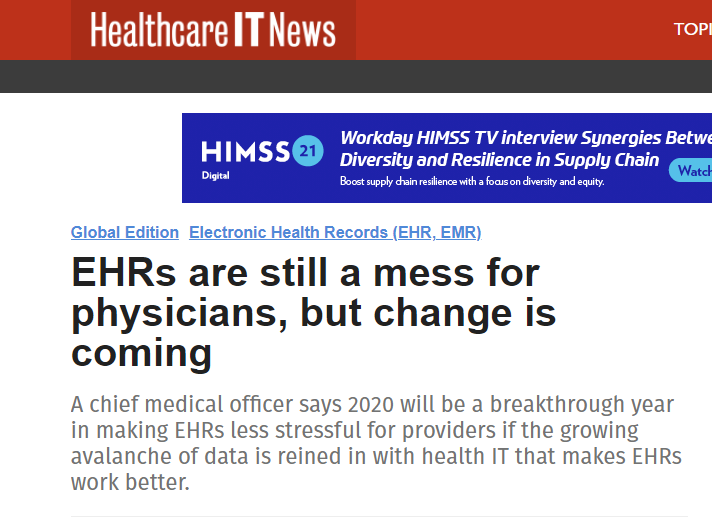
\includegraphics[scale=.4]{graphics/News Clip1.PNG}
\end{center}
\end{frame}

\begin{frame}{Physician Burnout}
\begin{center}
    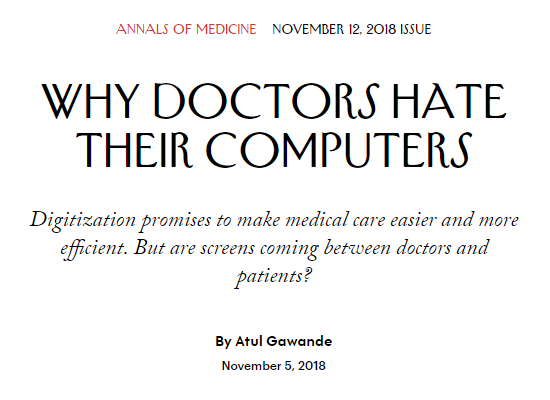
\includegraphics[scale=.5]{graphics/News Clip2.PNG}
\end{center}
\end{frame}

\begin{frame}{Physician Burnout}
\begin{center}
    
\includegraphics[scale=.3]{graphics/News Clip3.PNG}
\end{center}
\end{frame}

\begin{frame}{This Paper}

Does EHR implementation affect labor market decisions of physicians, specifically where, how much, and whether or not they work?
    
\end{frame}


\section{Contribution}

\begin{frame}{Branches of Literature}
\centering
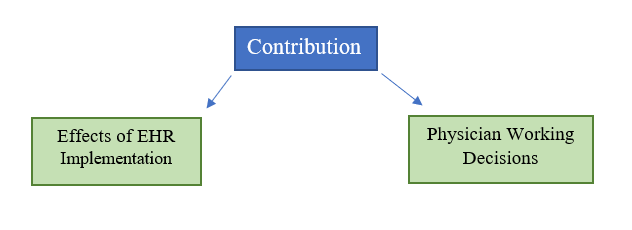
\includegraphics[scale=.45]{graphics/Contribution_litgraphic.PNG}

\end{frame}

\begin{frame}{Physician Labor Literature}
\centering
    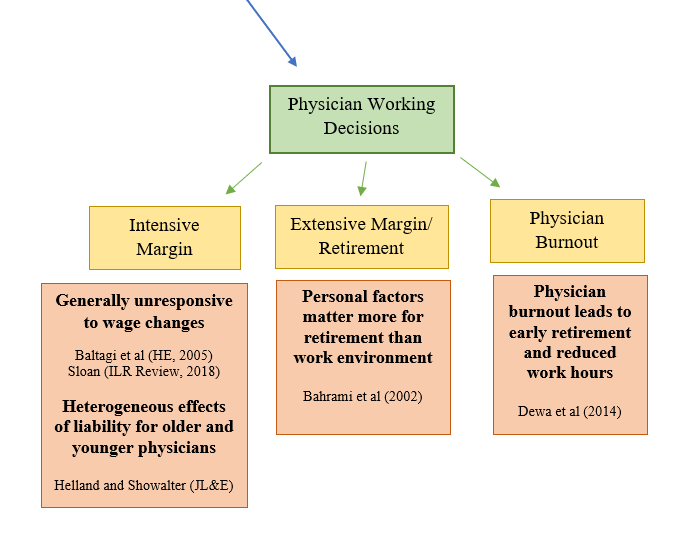
\includegraphics[scale=.45]{graphics/labor_litgraphic.PNG}
\end{frame}

\begin{frame}{EHR Literature}
    \centering
    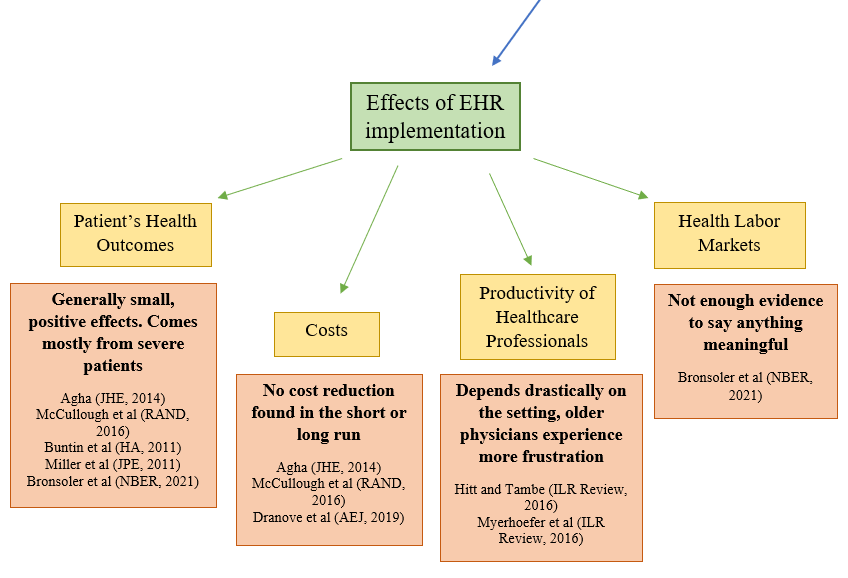
\includegraphics[scale=.45]{graphics/EHR_litgraphic.PNG}
\end{frame}


\section{Model}


\begin{frame}{Physician's Incentives}
\begin{itemize}
    \item Physician decides to work, possibly at a handful of hospitals
    \item Some proportion of these implement a new technology (an EHR)
    \item Two ways to think about the effect:
    \begin{enumerate}
        \item The EHR could impose a burden on the physician, leading them to shift work to other hospitals or lower workload
        \item The EHR could increase the physician's attachment to the implementing hospital, leading them to shift away from other hospitals and towards the EHR hospital
    \end{enumerate}
\end{itemize}
\end{frame}

\begin{frame}{Physician's Incentives: reduced form}
\begin{equation*}
    share_h=f()
\end{equation*}
    
\end{frame}

\begin{frame}{Variation in EHR Adoption}
\centering
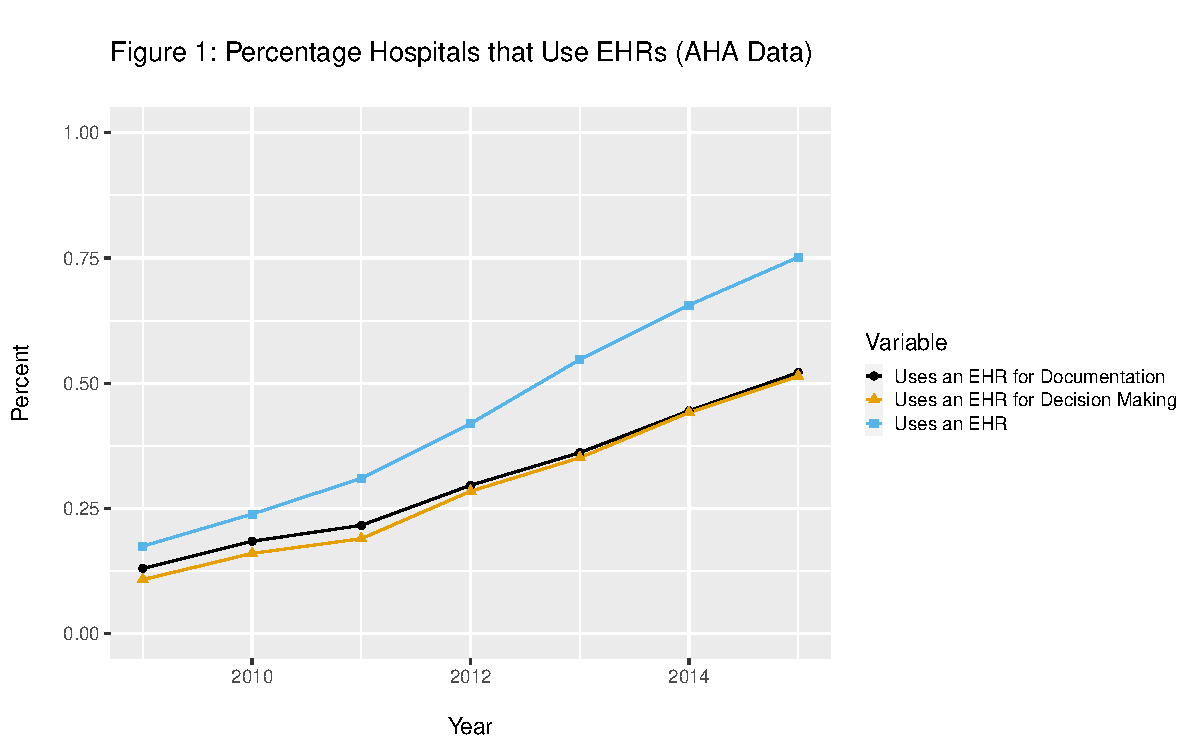
\includegraphics[scale=.55]{Objects/TYP_plot_hospEHR_year.pdf}
\end{frame}

\begin{frame}{Frame Title}
    
\end{frame}






\section{Plans}








\end{document}
